% This example is meant to be compiled with lualatex or xelatex

% The theme itself also supports pdflatex
\PassOptionsToPackage{unicode}{hyperref}
\documentclass[aspectratio=1610, 10pt]{beamer}

% Load packages you need here
\usepackage{polyglossia}
\setmainlanguage{german}
\usepackage[font=small,labelfont=bf]{caption}
\usepackage{csquotes}
\usepackage{siunitx}
\usepackage{subfigure}

\usepackage{amsmath}
\usepackage{amssymb}
\usepackage{mathtools}

\usepackage{hyperref}
\usepackage{bookmark}
\usepackage[absolute,overlay]{textpos}

%\usepackage[texcoord,
%grid,gridcolor=red!10,subgridcolor=green!10,gridunit=pt]
%{eso-pic}
% load the theme after all packages

\usetheme[
  showtotalframes, % show total number of frames in the footline
]{tudo}

% Put settings here, like
\unimathsetup{
  math-style=ISO,
  bold-style=ISO,
  nabla=upright,
  partial=upright,
  mathrm=sym,
}

\title{\Large{Cherenkov Detectors}}
\author[C.~Krause]{\normalsize{Christopher Krause}}
%\institute[E4]{\normalsize{Experimentelle Physik IV} \\ \normalsize{Fakultät Physik}}
\titlegraphic{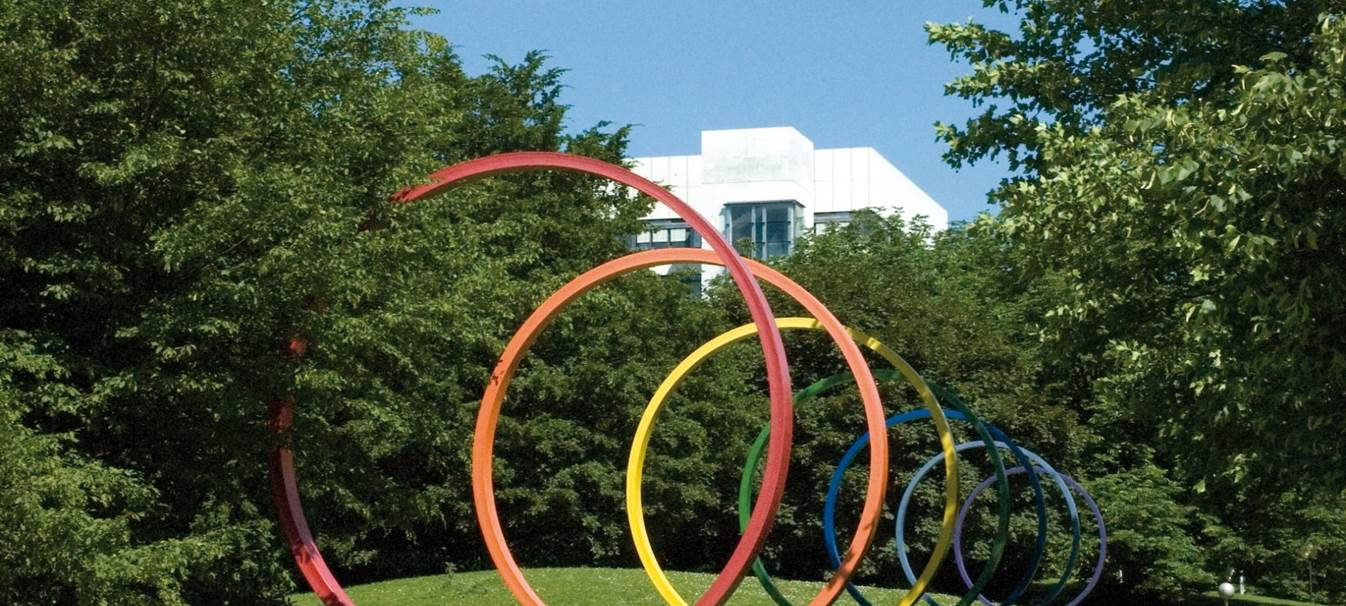
\includegraphics[width=0.67\textwidth]{images/tudo-title-2.jpg}}


\begin{document}

\maketitle


\begin{frame}{Cherenkov radiation}
  \begin{itemize}
    \item Discovered by Pavel Cherenkov in 1934 around a radioactive preparation in water (1958 Nobel Prize)
    \item Theory was developed in 1958 by Igor Tamm and Ilya Frank (1958 Nobel Prize)
    \item Electromagnetic radiation of a charged particle in a dielectric medium, which moves
    faster than the phase speed of light in that medium
  \end{itemize}
%  \begin{figure}
%      \includegraphics[width=0.53\textwidth]{images/interface.PNG}
%  \caption{Interface zur Berechnung von $N_{\mathrm{eff}}$ und $\alpha$.}
%  \end{figure}
\end{frame}


\end{document}
